\clearpage
\paragraph{Soggetto 2}~

Di seguito vengono presentate le misurazioni effettuate su un soggetto di sesso femminile, di età 41 anni e carnagione chiara. Il soggetto si trovava in condizioni di riposo.

\paragraph{MAX86916}~

Di seguito sono riportate le acquisizioni effettuate utilizzando il sensore MAX86916 su una finestra temporale di 10 secondi.

\subparagraph{Polpastrello indice sinistro}
Dalle acquisizioni riportate in figura \ref{fig:soggetto1_polpastrello}, effettuate sul polpastrello dell'indice della mano sinistra, si può notare come il segnale ottenuto sia di ottima qualità per tutte e quattro le lunghezze d'onda impiegate, confermando i risultati ottenuti con il soggetto 1, e anche le considerazioni fatte a livello teorico nel primo capitolo (vedi par. \ref{cap:sitimisura}). Infatti, dalle immagini riportate si possono distinguere chiaramente sia i picchi sistolici, quelli diastolici e le tacche dicrotiche. Anche qui si possono individuare 10 picchi del segnale, stimando una frequenza cardiaca di 60 battiti al minuto.
\begin{figure}[h]
	\centering
	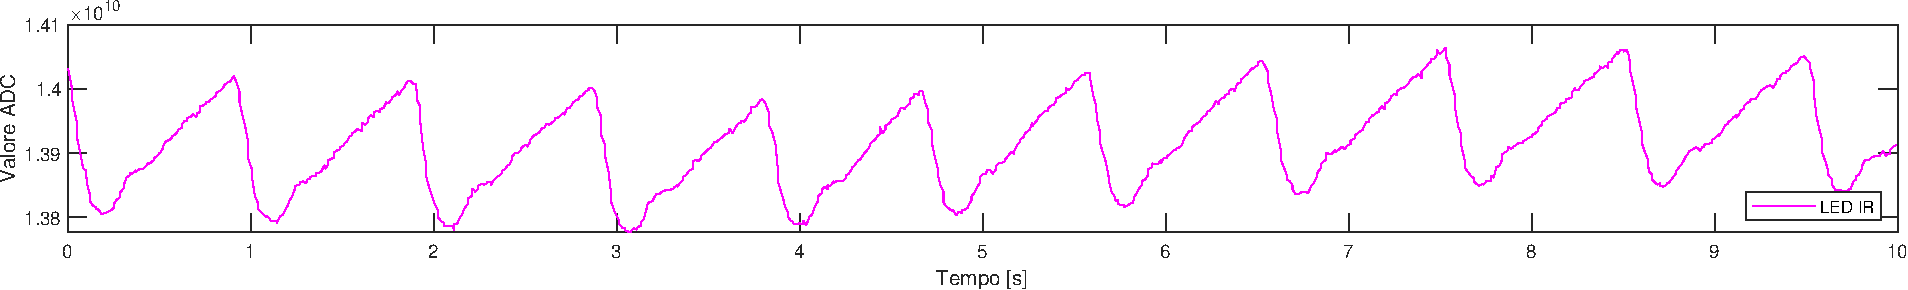
\includegraphics[width=1\linewidth]{ImageFiles/Misure Preliminari/Soggetto 2/max86916/polpastrello_ired}
	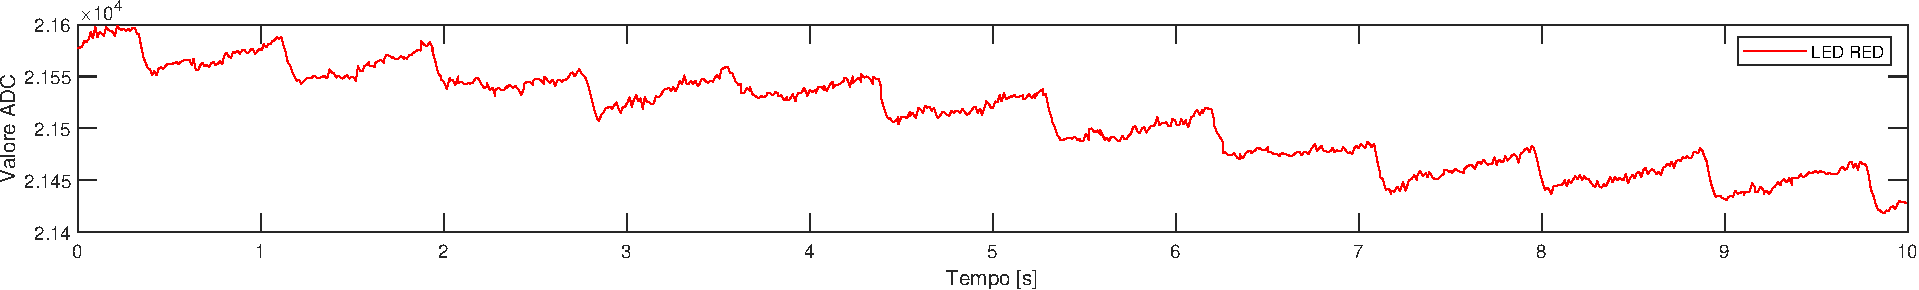
\includegraphics[width=1\linewidth]{ImageFiles/Misure Preliminari/Soggetto 2/max86916/polpastrello_red}
	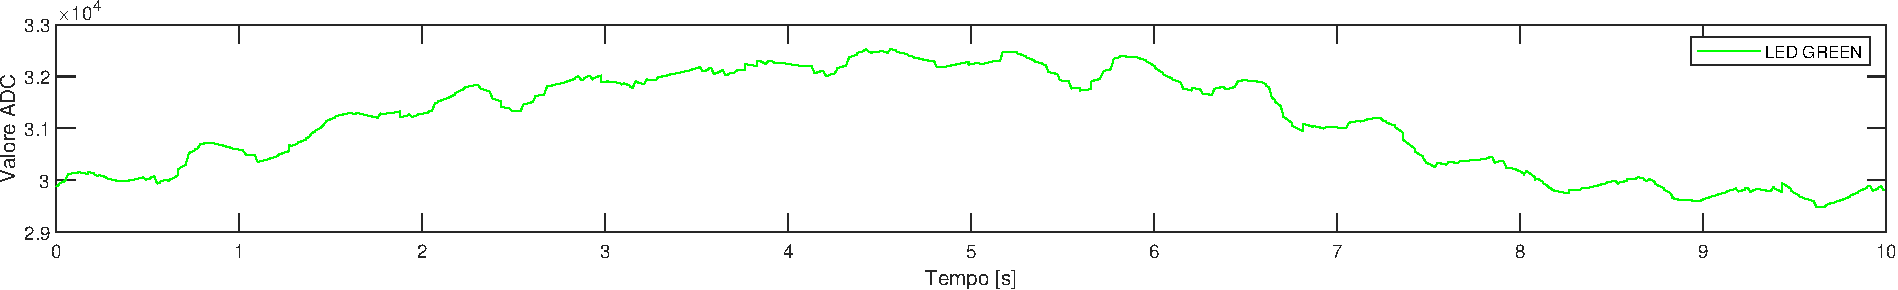
\includegraphics[width=1\linewidth]{ImageFiles/Misure Preliminari/Soggetto 2/max86916/polpastrello_green}
	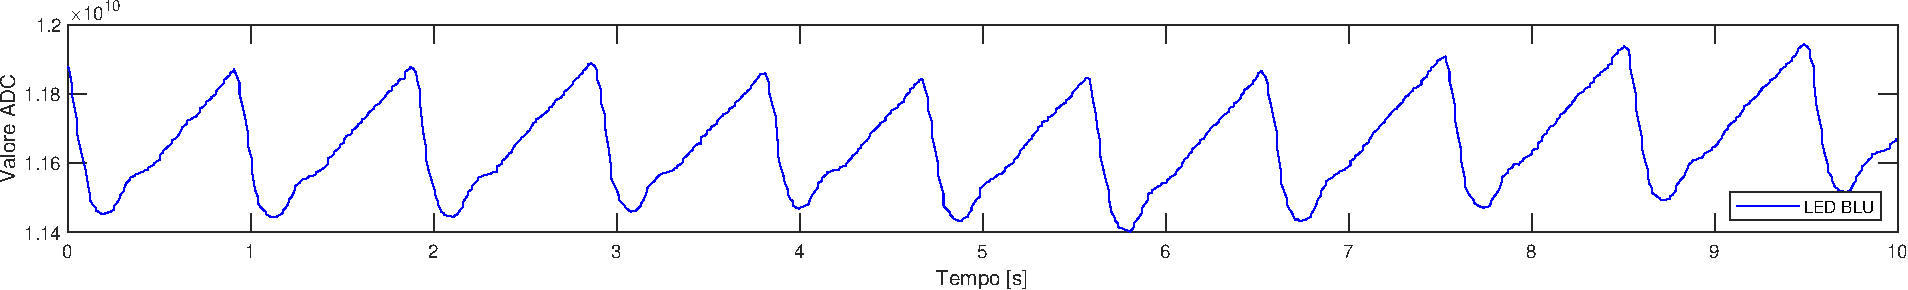
\includegraphics[width=1\linewidth]{ImageFiles/Misure Preliminari/Soggetto 2/max86916/polpastrello_blu}
	\caption{Soggetto 2 - MAX86916: segnali PPG acquisiti sul polpastrello del dito indice sinistro.}
	\label{fig:soggetto2_MAX86916_polpastrello}
\end{figure}

\subparagraph{Lobo orecchio sinistro}

Le acquisizioni ottenute sul lobo dell'orecchio sinistro presentano un segnale di qualità leggermente inferiore, principalmente dovuta alla difficoltà della misura in questo sito, a quella ottenuta con il polpastrello ma si tratta sempre di un ottimo segnale. Infatti, in figura \ref{fig:soggetto2_MAX86916_lobo}, si possono ancora apprezzare i picchi sistolici e diastolici su tutte le lunghezze d'onda impiegate. I picchi individuati sono 10, stimando una frequenza cardiaca di 60 battiti al minuto, coerente con il risultato ottenuto con la misura sul polpastrello.
\begin{figure}[h]
	\centering
	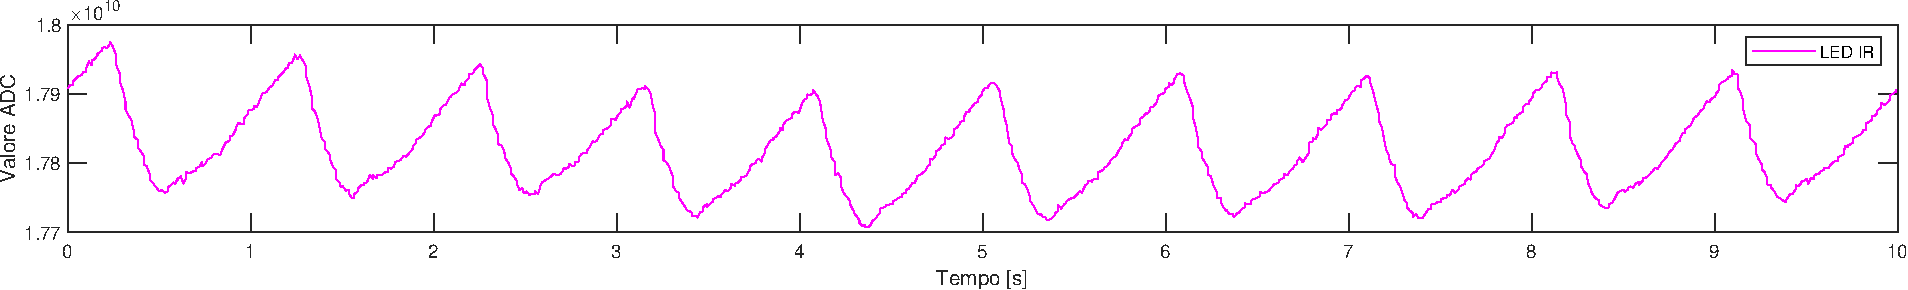
\includegraphics[width=1\linewidth]{ImageFiles/Misure Preliminari/Soggetto 2/max86916/lobo_ired}
	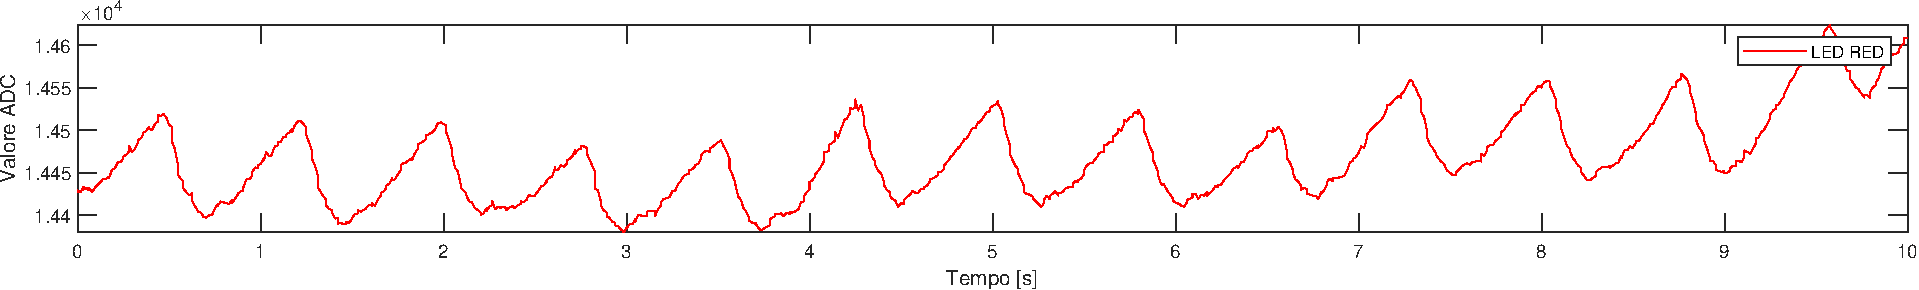
\includegraphics[width=1\linewidth]{ImageFiles/Misure Preliminari/Soggetto 2/max86916/lobo_red}
	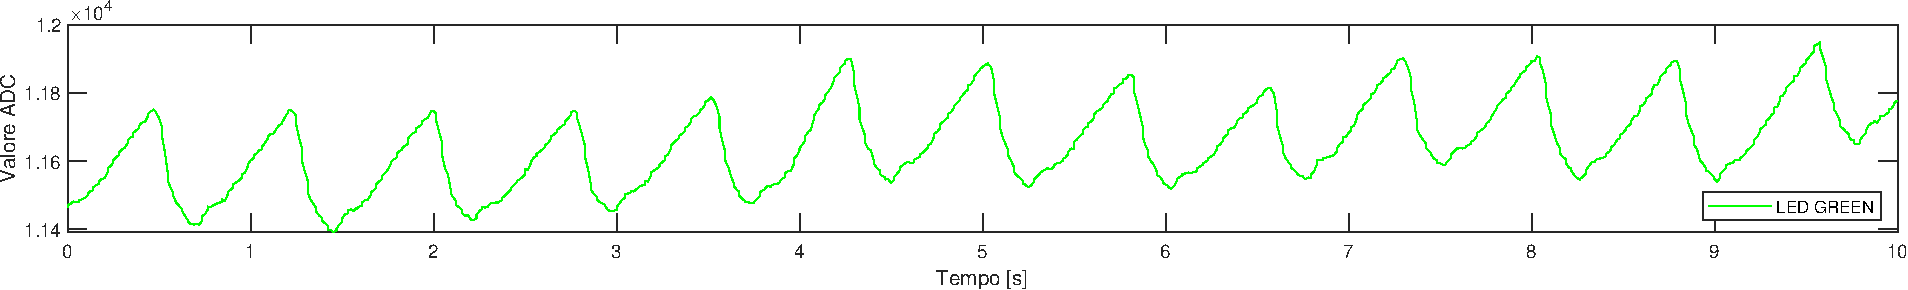
\includegraphics[width=1\linewidth]{ImageFiles/Misure Preliminari/Soggetto 2/max86916/lobo_green}
	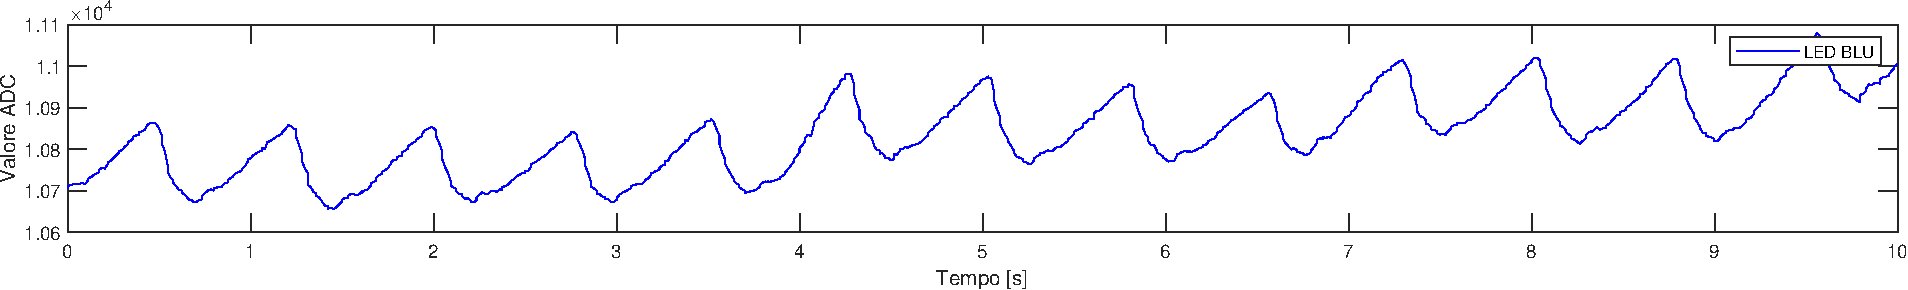
\includegraphics[width=1\linewidth]{ImageFiles/Misure Preliminari/Soggetto 2/max86916/lobo_blu}
	\caption{Soggetto 2 - MAX86916: segnali PPG acquisiti sul lobo dell'orecchio destro.}
	\label{fig:soggetto2_MAX86916_lobo}
\end{figure}

\subparagraph{Polso antero-interno sinistro}

Le misure effettuate sulla zona del polso antero-interno sono più soggette a disturbi, principalmente dovute sempre a movimenti di natura involontaria. Come si può vedere in figura \ref{fig:soggetto2_MAX86916_polso}, questi disturbi sono più visibili per la luce rossa e infrarossa, mentre per la luce blu e verde il segnale si dimostra ancora pulito e chiaro. Nonostante ciò la qualità si può reputare buona, infatti sono ancora individuabili i picchi di interesse. La frequenza cardiaca stimata da questa acquisizione è di 63 battiti al minuto.
\begin{figure}[h]
	\centering
	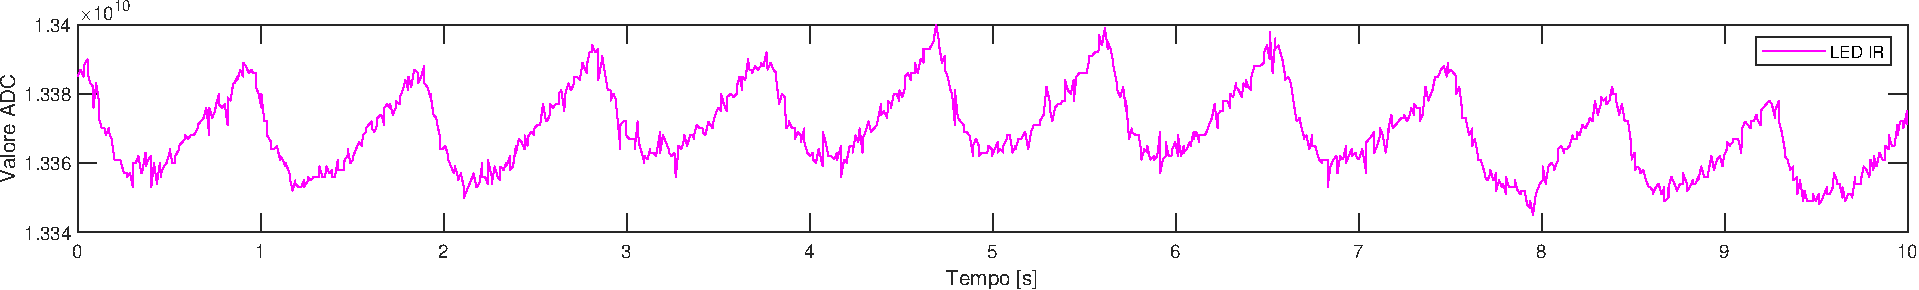
\includegraphics[width=1\linewidth]{ImageFiles/Misure Preliminari/Soggetto 2/max86916/polso_inferiore_ired}
	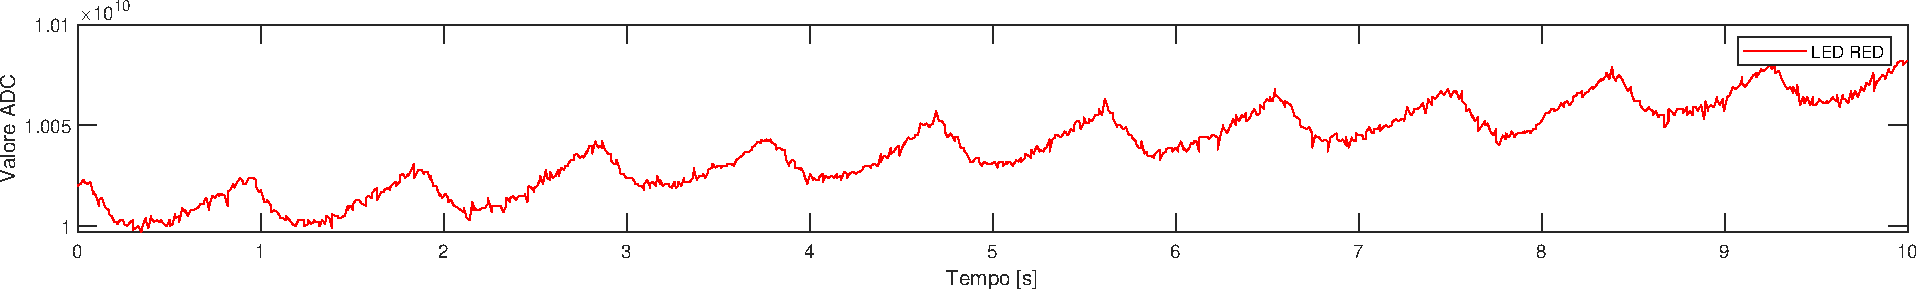
\includegraphics[width=1\linewidth]{ImageFiles/Misure Preliminari/Soggetto 2/max86916/polso_inferiore_red}
	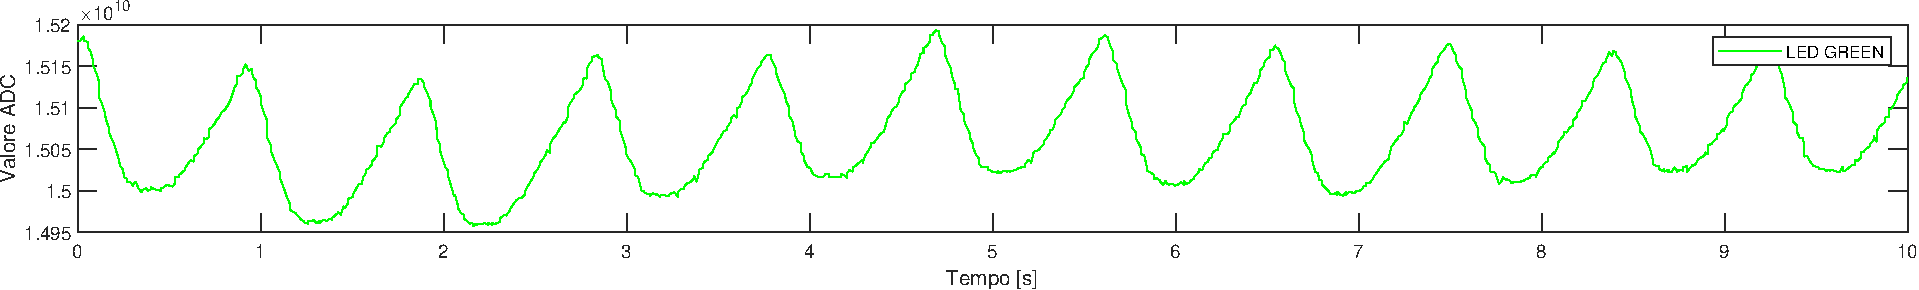
\includegraphics[width=1\linewidth]{ImageFiles/Misure Preliminari/Soggetto 2/max86916/polso_inferiore_green}
	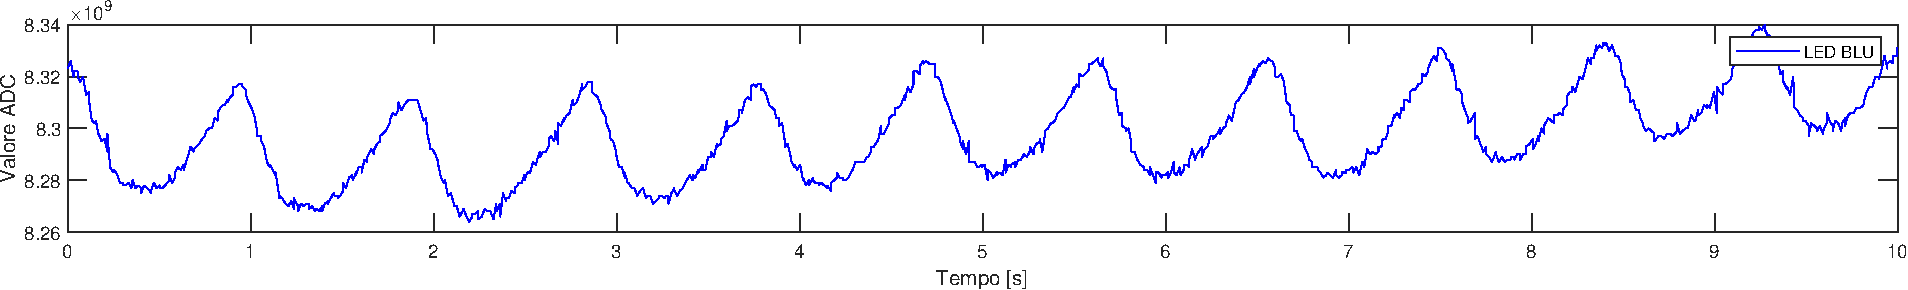
\includegraphics[width=1\linewidth]{ImageFiles/Misure Preliminari/Soggetto 2/max86916/polso_inferiore_blu}
	\caption{Soggetto 2 - MAX86916: segnali PPG acquisiti sul polso destro.}
	\label{fig:soggetto2_MAX86916_polso}
\end{figure}

\subparagraph{Fronte}

Infine,in figura \ref{fig:soggetto2_MAX86916_lobo}, vengono riportati i risultati delle acquisizioni effettuate sulla fronte. I segnali ottenuti dalle lunghezze d'onda rossa e infrarossa presentano una qualità, mentre non vale lo stesso per le lunghezze d'onda blu e verde. Infatti, per queste ultime si possono ancora distinguere i picchi massimi, mentre quelli sistolici e diastolici sono più difficili da individuare. La frequenza cardiaca stimata è di 60 battiti al minuto, confermando i precedenti risultati.

\begin{figure}[h]
	\centering
	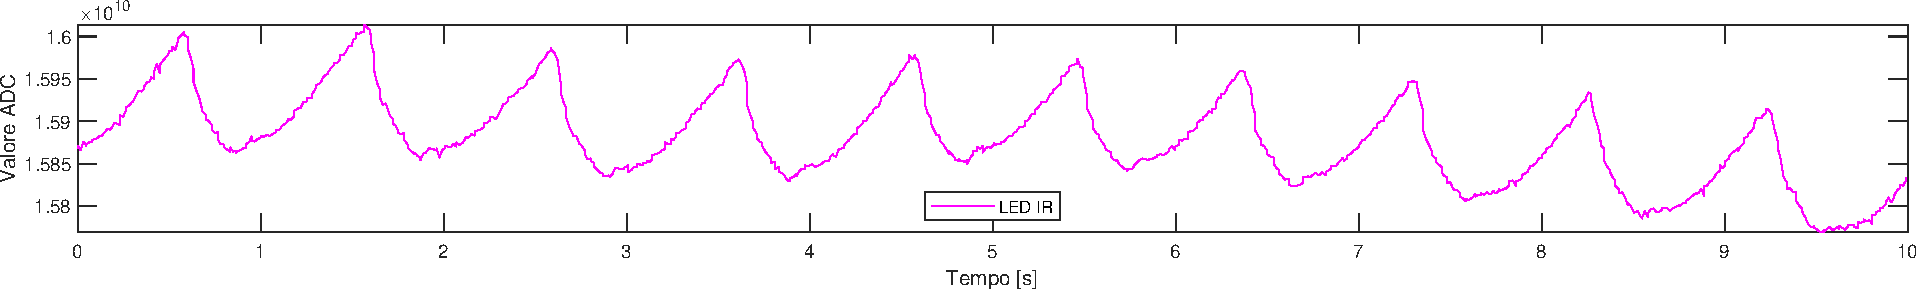
\includegraphics[width=1\linewidth]{ImageFiles/Misure Preliminari/Soggetto 2/max86916/fronte_ired}
	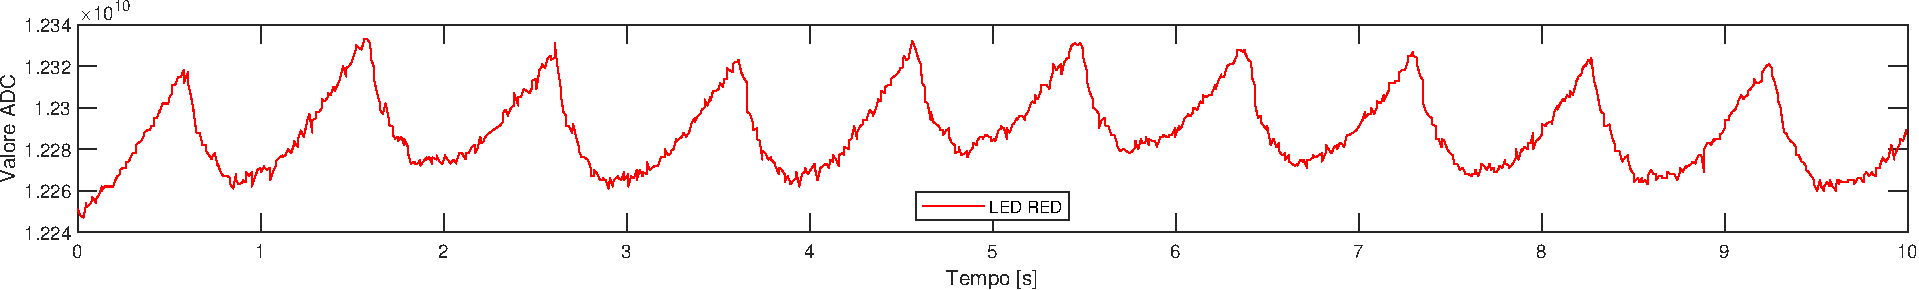
\includegraphics[width=1\linewidth]{ImageFiles/Misure Preliminari/Soggetto 2/max86916/fronte_red}
	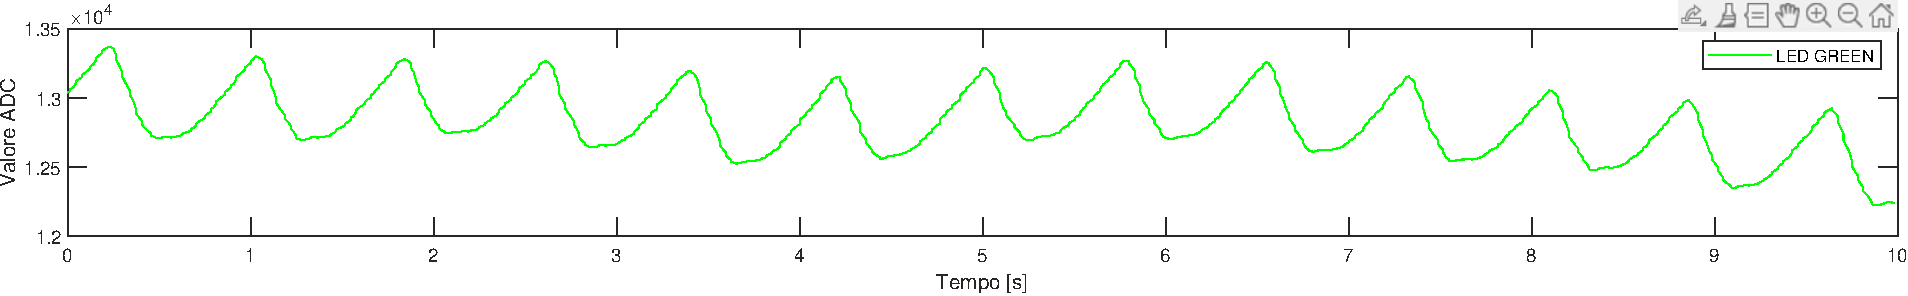
\includegraphics[width=1\linewidth]{ImageFiles/Misure Preliminari/Soggetto 2/max86916/fronte_green}
	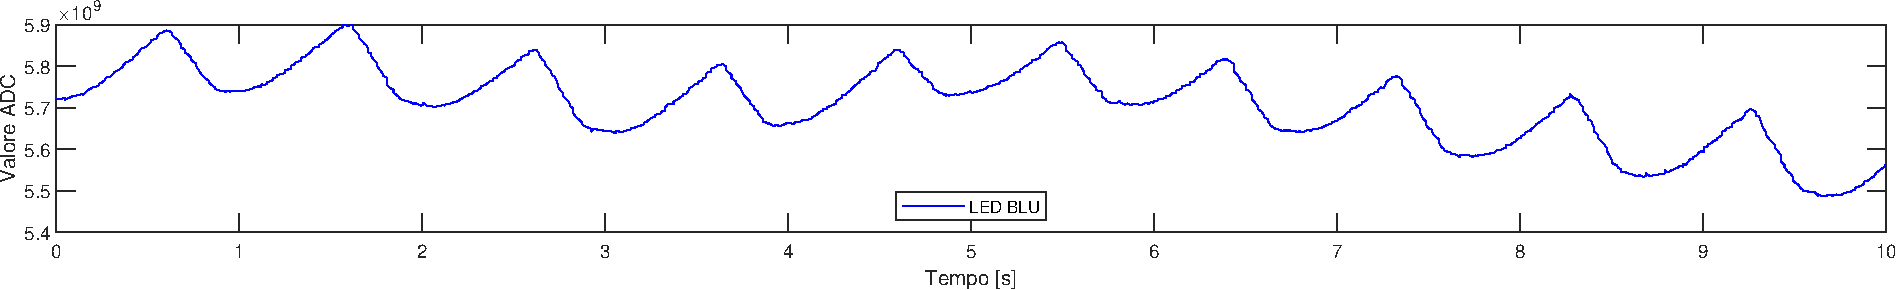
\includegraphics[width=1\linewidth]{ImageFiles/Misure Preliminari/Soggetto 2/max86916/fronte_blu}
	\caption{Soggetto 2 - MAX86916: segnali PPG acquisiti sulla fronte.}
	\label{fig:soggetto2_MAX86916_fronte}
\end{figure}

\clearpage

\paragraph{MAXM86161}~

Di seguito sono riportate le acquisizioni effettuate utilizzando il sensore MAXM86161 su una finestra temporale di 10 secondi.

\subparagraph{Polpastrello indice sinistro}
\begin{figure}[h]
	\centering
	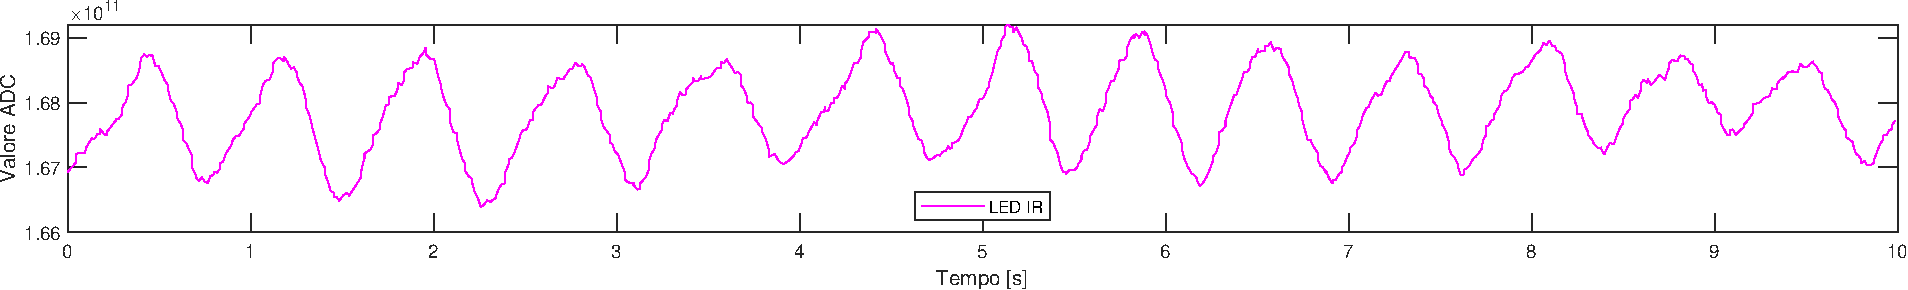
\includegraphics[width=1\linewidth]{ImageFiles/Misure Preliminari/Soggetto 2/maxm86161/polpastrello_ir_moving_avg}
	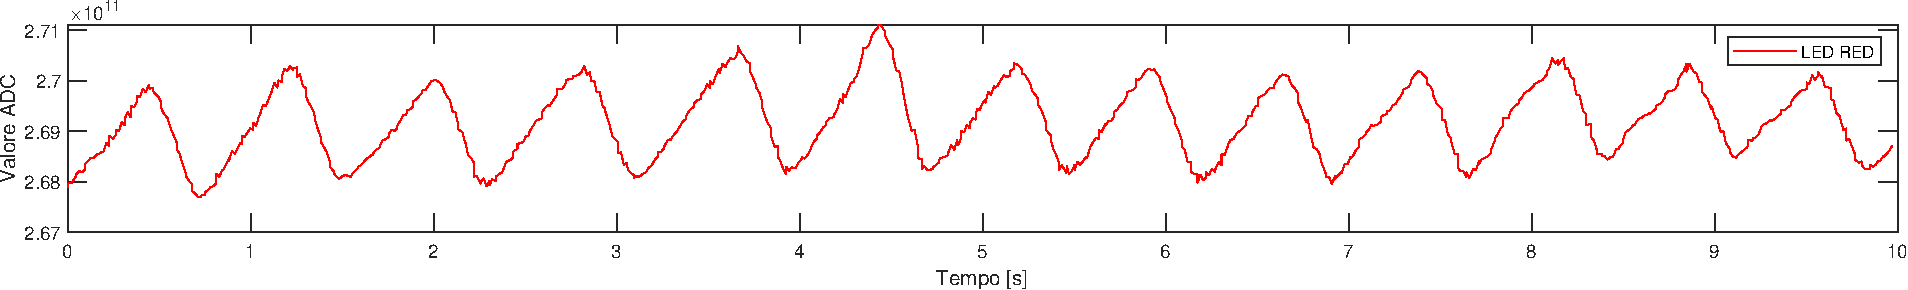
\includegraphics[width=1\linewidth]{ImageFiles/Misure Preliminari/Soggetto 2/maxm86161/polpastrello_red_moving_avg}
	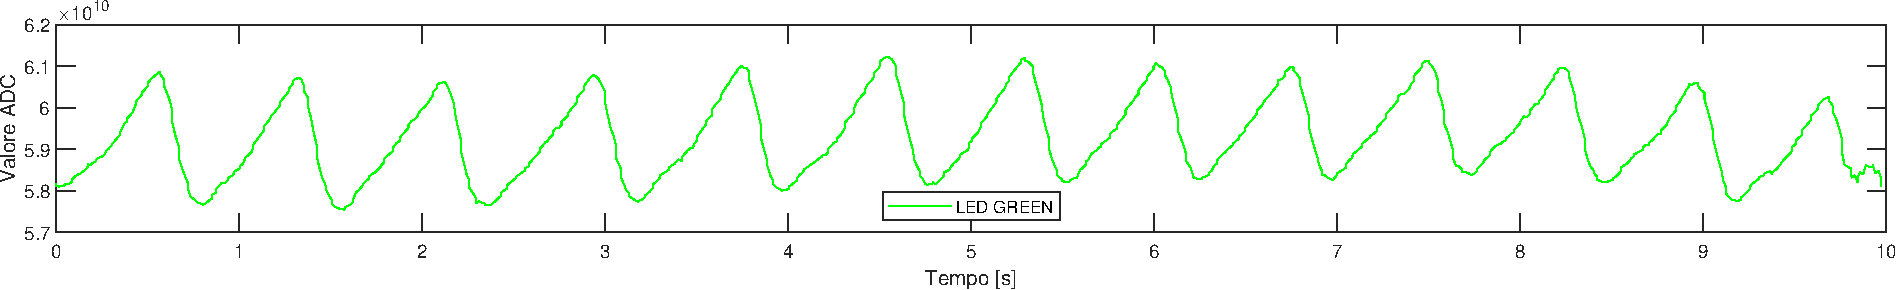
\includegraphics[width=1\linewidth]{ImageFiles/Misure Preliminari/Soggetto 2/maxm86161/polpastrello_green_moving_avg}
	\caption{Soggetto 2 - MAXM86161: segnali PPG acquisiti sul polpastrello del dito indice sinistro.}
	\label{fig:soggetto2_MAXM86161_polpastrello}
\end{figure}

\subparagraph{Lobo orecchio sinistro}
\begin{figure}[h]
	\centering
	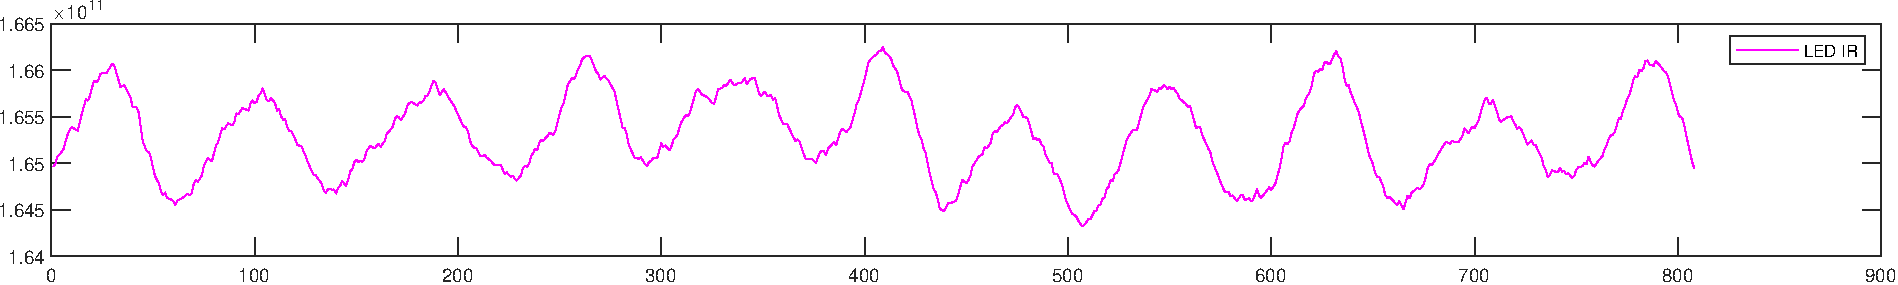
\includegraphics[width=1\linewidth]{ImageFiles/Misure Preliminari/Soggetto 2/maxm86161/lobo_ir_moving_avg}
	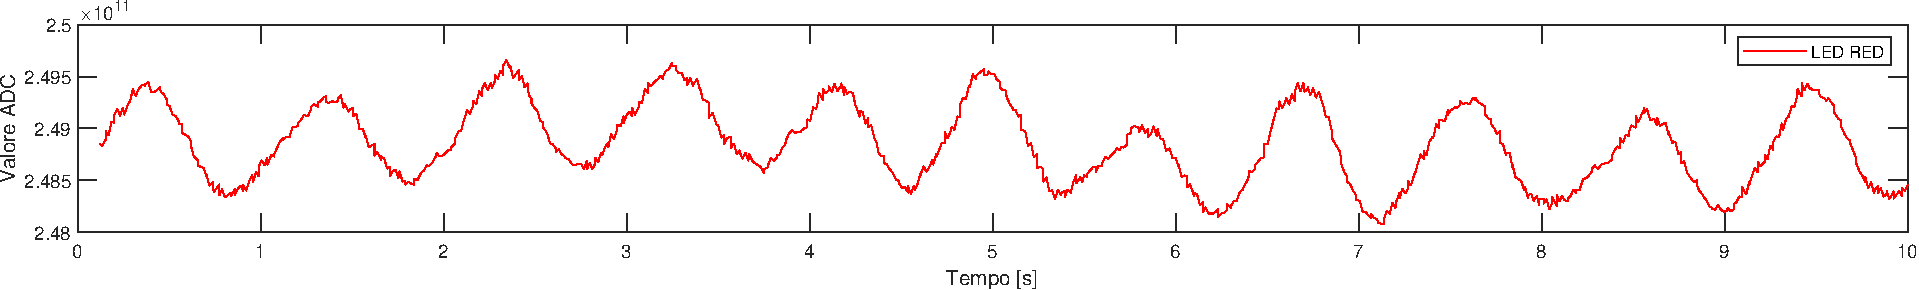
\includegraphics[width=1\linewidth]{ImageFiles/Misure Preliminari/Soggetto 2/maxm86161/lobo_red_moving_avg}
	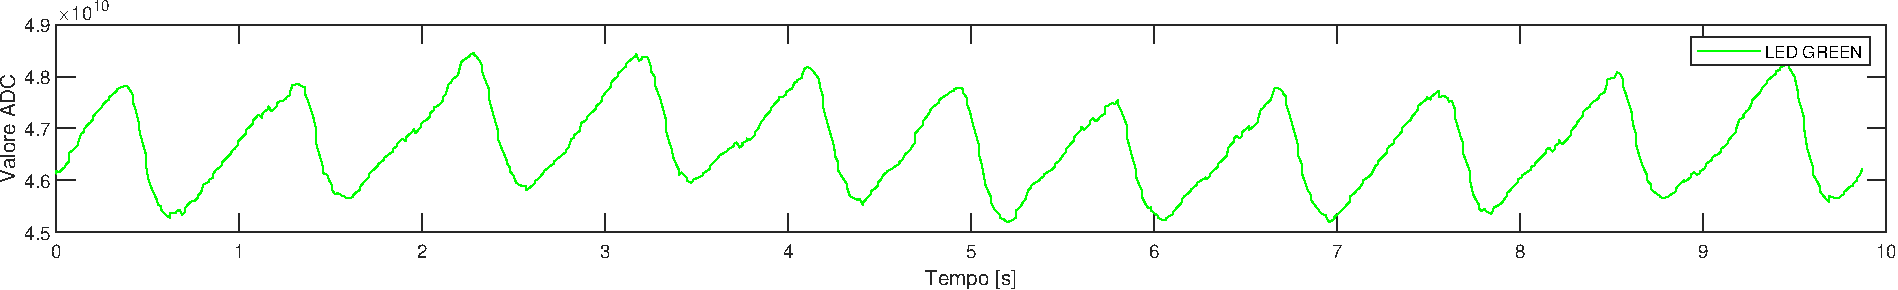
\includegraphics[width=1\linewidth]{ImageFiles/Misure Preliminari/Soggetto 2/maxm86161/lobo_green_moving_avg}
	\caption{Soggetto 2 - MAXM86161: segnali PPG acquisiti sul lobo dell'orecchio destro.}
	\label{fig:soggetto2_MAXM86161_lobo}
\end{figure}

\subparagraph{Polso antero-interno sinistro}
\begin{figure}[h]
	\centering
	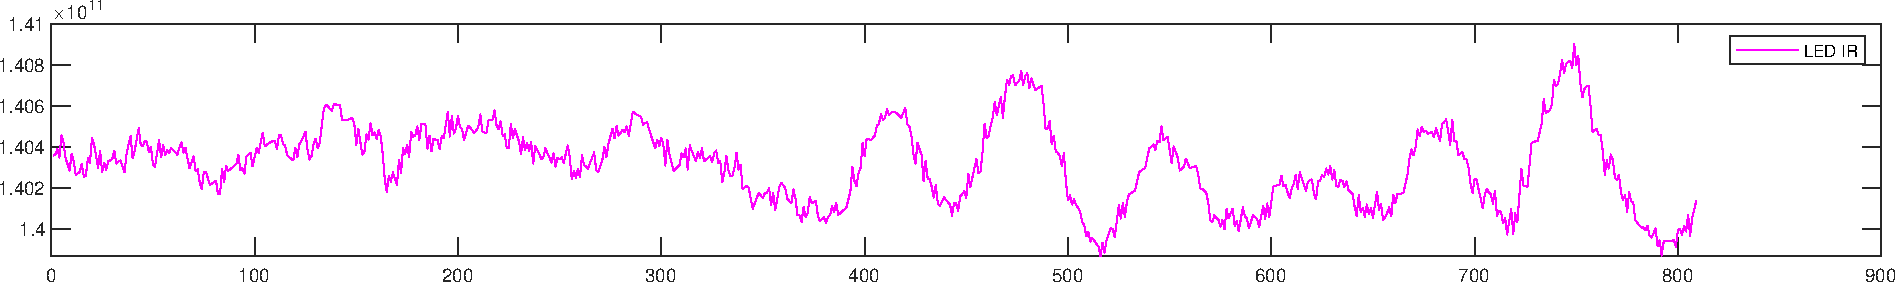
\includegraphics[width=1\linewidth]{ImageFiles/Misure Preliminari/Soggetto 2/maxm86161/polso_inferiore_ir_moving_avg}
	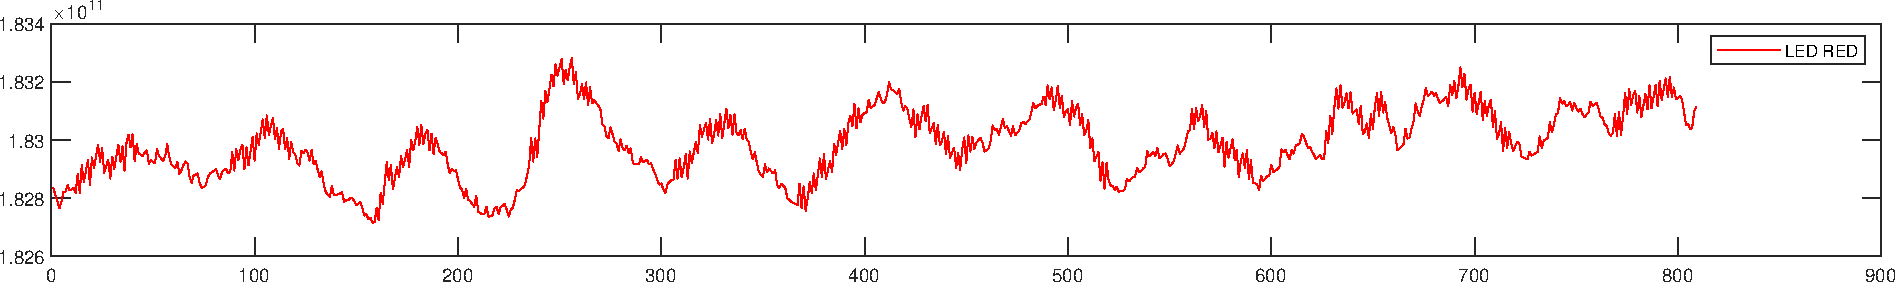
\includegraphics[width=1\linewidth]{ImageFiles/Misure Preliminari/Soggetto 2/maxm86161/polso_inferiore_red_moving_avg}
	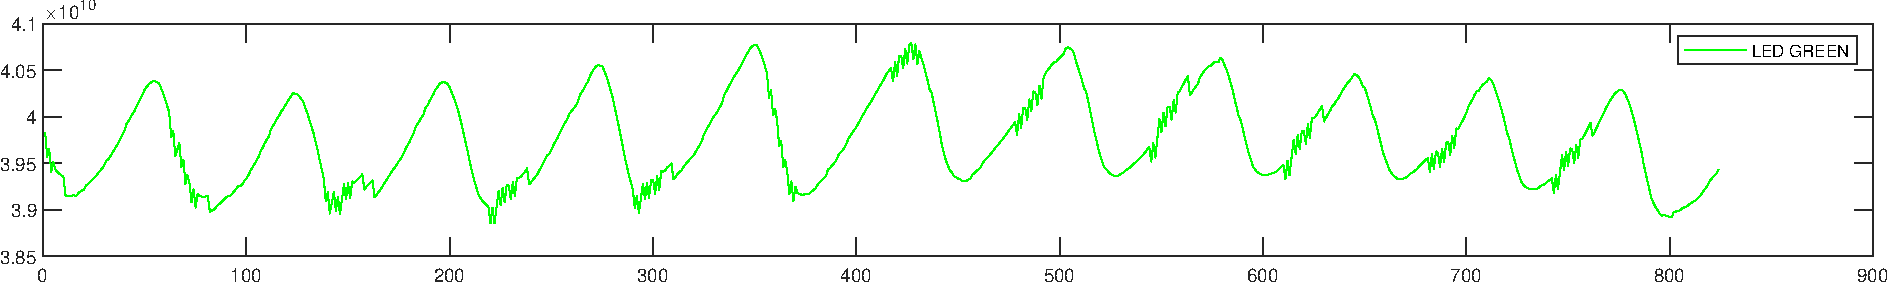
\includegraphics[width=1\linewidth]{ImageFiles/Misure Preliminari/Soggetto 2/maxm86161/polso_inferiore_green_moving_avg}
	\caption{Soggetto 2 - MAXM86161: segnali PPG acquisiti sul polso destro.}
	\label{fig:soggetto2_MAXM86161_polso}
\end{figure}

\subparagraph{Fronte}

\begin{figure}[h]
	\centering
	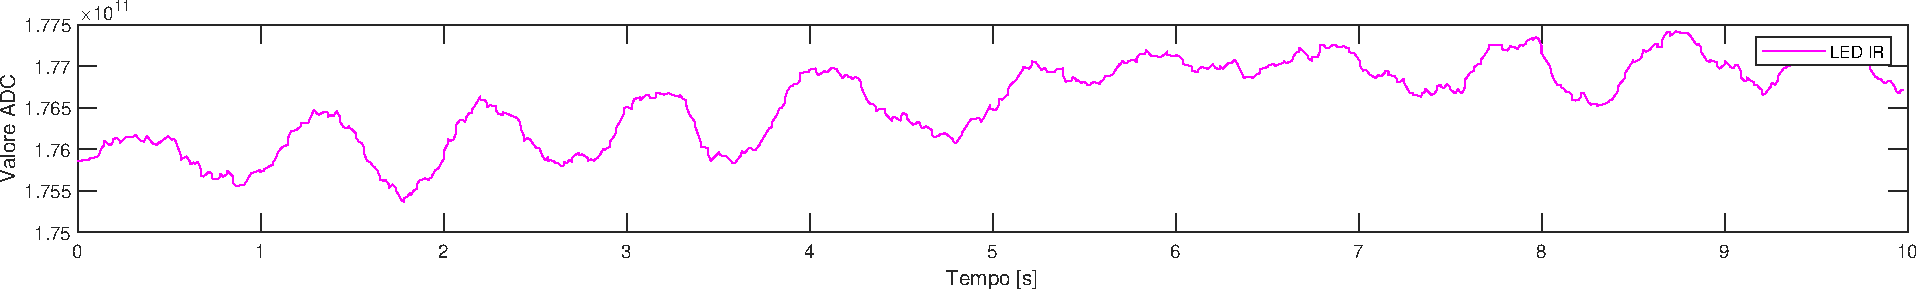
\includegraphics[width=1\linewidth]{ImageFiles/Misure Preliminari/Soggetto 2/maxm86161/fronte_ir_moving_avg}
	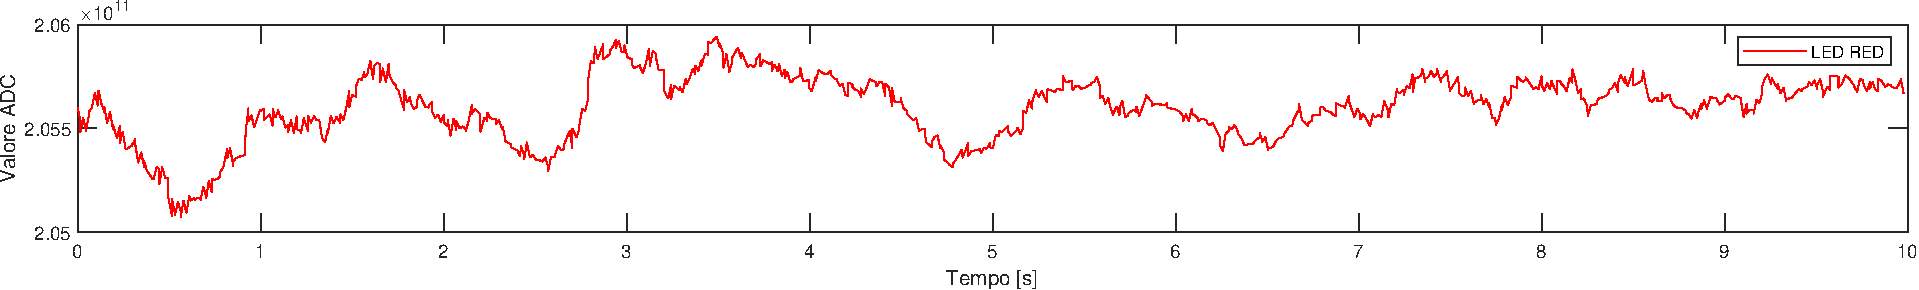
\includegraphics[width=1\linewidth]{ImageFiles/Misure Preliminari/Soggetto 2/maxm86161/fronte_red_moving_avg}
	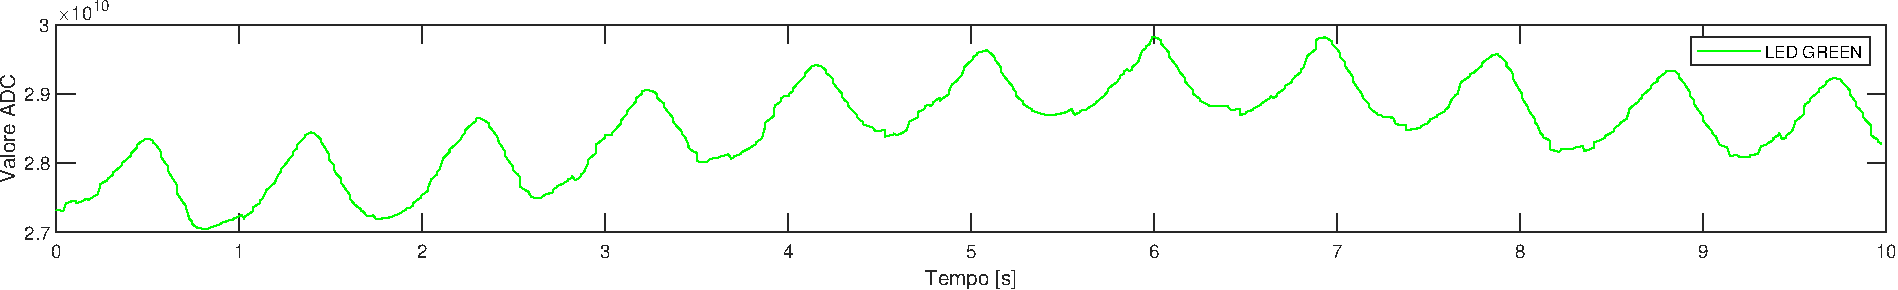
\includegraphics[width=1\linewidth]{ImageFiles/Misure Preliminari/Soggetto 2/maxm86161/fronte_green_moving_avg}
	\caption{Soggetto 2 - MAXM86161: segnali PPG acquisiti sulla fronte.}
	\label{fig:soggetto2_MAXM86161_fronte}
\end{figure}


\clearpage